\section{Deciphering Spanish Gigaword}
\label{decipher_spanish}

In this section, we describe our data and experimental conditions for deciphering Spanish into English.

\subsection{Data}

In our Spanish/English decipherment experiments, we use half of the Gigaword corpus as monolingual data, and a small amount of parallel data from Europarl {\em for evaluation}. We keep only the 10k most frequent word types for both languages and replace all other word types with ``UNK''.  We also exclude sentences longer than 40 tokens, which significantly slow down our parser. After preprocessing, the size of data for each language is shown in Table~\ref{es-en-data}. 
%The Gigaword corpus consists of news articles from different news agencies.  
While we use all the monolingual data shown in Table \ref{es-en-data} to learn word embeddings, we only parse the AFP (Agence France-Presse) section of the Gigaword corpus to extract cipher dependency bigrams and build a plaintext language model. We also use GIZA \cite{GIZA} to align Europarl parallel data to build a dictionary for evaluating our decipherment.

 \begin{table}
 \begin{center}
 \begin{tabular}{ |c|c|c| } \hline
             & Spanish & English \\ \hline
\multirow{2}{*}{Training} & 992 million & 940 million \\ 
 & (Gigaword) & (Gigaword)  \\ \hline
\multirow{2}{*}{Evaluation} & 1.1 million & 1.0 million \\
 & (Europarl) & (Europarl) \\ \hline
 \end{tabular}
 \caption{Size of data in tokens used in Spanish/English decipherment experiment}
 \label{es-en-data}
 \end{center}
 \end{table}

\subsection{Systems}

We implement a baseline system based on the work described in \newcite{dou-knight:2013:EMNLP}. The baseline system carries out decipherment on dependency bigrams.  Therefore, we use the Bohnet parser \cite{bohnet:2010:PAPERS} to parse the AFP section of both Spanish and English versions of the Gigaword corpus. Since not all dependency relations are shared across the two languages, we do not extract all dependency bigrams. Instead, we only use bigrams with dependency relations from the following list: 

\begin{itemize}
\item Verb / Subject
\item Verb / Object
\item Preposition / Object
\item Noun / Noun-Modifier
\end{itemize}

%The baseline uses slice sampling with a uniform base distribution.
We denote the system that uses our new method as \textbf{DMRE} (Dirichlet Multinomial Regression with Embedings). The system is the same as the baseline except that it uses a base distribution derived from word embeddings similarities. Word embeddings are learned using word2vec \cite{mikolov2013efficient}.

For all the systems, language models are built using the SRILM toolkit \cite{srilm}. We use the modified Kneser-Ney \cite{KneserNey95} algorithm for smoothing.


\subsection{Sampling Procedure}
\label{sample_procedure}

 \begin{figure}[!ht]
  \centering
  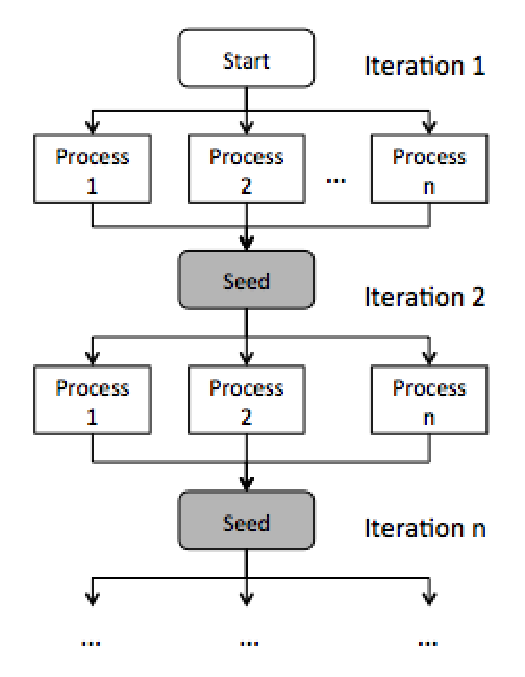
\includegraphics[width=2.9in,height=3.8in]{iterative_sampling}
  \caption{Iterative sampling procedures}
\label{iterative_sampling}
\end{figure}

Motivated by the previous work, we use multiple random restarts and an iterative sampling process to improve decipherment \cite{Dou:2012}. As shown in Figure~\ref{iterative_sampling}, we start a few sampling processes each with a different random sample. Then results from different runs are combined to initiate the next sampling iteration. The details of the sampling procedure are listed below:

 \begin{enumerate}
  \item Extract dependency bigrams from parsing outputs and collect their counts.
  \item Keep bigrams whose counts are greater than a threshold $t$. Then start N different randomly seeded and initialized sampling processes. Perform sampling.
  \item At the end of sampling, extract word translation pairs $(f,e)$ from the final sample. Estimate translation probabilities $P(e|f)$ for each pair. Then construct a translation table by keeping translation pairs $(f,e)$ seen in more than one decipherment and use the average $P(e|f)$ as the new translation probability.
  \item Start N different sampling processes again. Initialize the first samples with the translation pairs obtained from the previous step (for each dependency bigram $f_{1},f_{2}$, find an English sequence $e_{1},e_{2}$, whose $P(e_{1}|f_{1})\cdot P(e_{2}|f_{2})\cdot P(e_{1},e_{2})$is the highest). Initialize similarity matrix $M$ with one learned by previous sampling process whose posterior probability is highest. Go to the third step, repeat until it converges.
  \item Lower the threshold $t$ to include more bigrams into the sampling process. Go to the second step, and repeat until $t=1$.
 \end{enumerate}

The sampling process consists of sampling and learning of similarity matrix $M$. The sampling process creates training examples for learning $M$, and the new $M$ is used to update the base distribution for sampling. In our Spanish/English decipherment experiments, we use 10 different random starts. As pointed out in section~\ref{sec:theory}, setting $\alpha_{\plain}$ to it's theoretical value (equation~\ref{base-concentration}) gives poor results as it can be quite large. In experiments, we set $\alpha_{\plain}$ to a small value for the smaller data sets and increase it as more ciphtertext becomes available. We find that using the learned base distribution always improves decipherment accuracy, however, certain ranges are better for a given data size. We find that $\alpha_{\plain}$ values of $1, 2$, and $5$ for ciphertexts with 100k, 1 million, and 10 million tokens respectively works well for decipherment. 

\section{Deciphering Malagasy}
\label{decipher_malagasy}

%In this section, we first introduce the Malagasy language, and describe the data used in the experiments; then explain what makes deciphering Malagasy more challenging compared with Spanish, and differences in experiment settings for achieving higher decipherment accuracy.
% need to maintain anonymity
%\subsection{The Malagasy Language}

Despite spoken in Africa, Malagasy has its root in Asia, and belongs to the Malayo-Polynesian branch of the Austronesian language family. Malagasy and English have very different word order (VOS versus SVO). Generally, Malagasy is a typical head-initial language: Determiners precede nouns, while other modifiers and relative clauses follow nouns (e.g. ny ``the'' ankizilahy ``boy'' kely ``little''). The significant differences in word order pose great challenges for both parsing and decipherment.


\subsection{Data}

Table~\ref{mlg-en-data} lists the sizes of monolingual and parallel data used in this experiment, released by \newcite{dou-vaswani-knight:2014:EMNLP2014}. The monolingual data in Malagasy contains news text collected from Madagascar websites. The English monolingual data contains Gigaword and an additional 300 million tokens of African news. Parallel data (used for evaluation only) is collected from GlobalVoices, a multilingual news website, where volunteers translate news into different languages.

 \begin{table}
 \begin{center}
 \begin{tabular}{ |c|c|c| } \hline
             & Malagasy & English \\ \hline
\multirow{2}{*}{Training} & 16 million & 1.2 billion\\ 
& (Web) & \pbox{2cm}{ (Gigaword \\ and Web)}  \\ \hline
\multirow{2}{*}{Evaluation} & 2.0 million& 1.8 million \\
 & (GlobalVoices) & (GlobalVoices)  \\ \hline
 \end{tabular}
 \caption{Size of data in tokens used in Malagasy/English decipherment experiment. GlobalVoices is a parallel corpus.}
 \label{mlg-en-data}
 \end{center}
 \end{table}
 
\subsection{Systems}
The baseline system is the same as the baseline used in Spanish/English decipherment experiments. We use data provided in previous work \cite{dou-vaswani-knight:2014:EMNLP2014} to build a Malagasy dependency parser. For English, we use the Turbo parser, trained on the Penn Treebank \cite{TurboParser}.  

Because the Malagasy parser does not predict dependency relation types, we use the following head-child part-of-speech (POS) tag patterns to select a subset of dependency bigrams for decipherment: 
%We list the selected POS tag patterns in Table \ref{mlg-en-dep-type}.

% keep format same as previous section on Spanish.

\begin{itemize}
\item Verb / Noun
\item Verb / Proper Noun
\item Verb / Personal Pronoun
\item Preposition / Noun
\item Preposision / Proper Noun
\item Noun / Adjective
\item Noun / Determiner
\item Noun / Verb Particle
\item Noun / Verb Noun % what is this?
\item Noun / Cardinal
\item Noun / Noun
\end{itemize}

%
% \begin{table}
% \begin{center}
% \begin{tabular}{ |c|c| } \hline
%          Head POS & Child POS \\ \hline
%Verb & Noun \\ \hline
%Verb & Proper Noun \\ \hline
%Verb & Person Pronoun \\ \hline
%Preposition & Noun \\ \hline
%Preposition & Proper Noun \\ \hline
%Noun & Adjective \\ \hline
%Noun & Determiner \\ \hline
%Noun & Verb Particle \\ \hline
%Noun & Verb Noun \\ \hline
%Noun & Cardinal Number \\ \hline
%Noun & Noun \\ \hline
% \end{tabular}
% \caption{Head-Child POS patterns used in decipherment}
% \label{mlg-en-dep-type}
% \end{center}
% \end{table}
%

\subsection{Sampling Procedure}

We use the same sampling protocol designed for Spanish/English decipherment. We double the number of random starts to 20. Further more, compared with Spanish/English decipherment, we find the base distribution plays a more important role in achieving higher decipherment accuracy for Malagasy/English. Therefore, we set $\alpha$ to 10, 50, and 200 when deciphering 100k, 1 million, and 20 million token ciphtertexts, respectively.


\section{Results}

%
 \begin{table*}[!ht]
 \begin{center}
 \begin{tabular}{ |c|c|c|c|c|c|c|c|c| } \hline
         & \multicolumn{4}{|c|}{Spanish/English} & \multicolumn{4}{|c|}{Malagasy/English} \\ \hline
 Top &  \multicolumn{2}{|c|}{5k} & \multicolumn{2}{|c|}{10k} & \multicolumn{2}{|c|}{5k} & \multicolumn{2}{|c|}{10k} \\ \hline
 System &  Baseline & DMRE & Baseline & DMRE &  Baseline & DMRE & Baseline & DMRE \\ \hline
 100k &  1.9 & 12.4 & 1.1 & 7.1 &  1.2 & 2.7 & 0.6 & 1.4 \\ \hline
 1 million &  7.3 & 37.7& 4.2 & 23.6 &  2.5 & 5.8 & 1.3 & 3.2 \\ \hline
 10 million &  29.0 & 64.7 & 15.9 & 43.7 &  5.4 & 11.2 & 3.0 & 6.9 \\ \hline
 \end{tabular}
 \caption{Spanish/English, Malagasy/English decipherment top-5 accuracy (\%) of 5k and 10k most frequent word types}
 \label{decipher-acc-result}
 \end{center}
 \end{table*}
%

In this section, we first compare decipherment accuracy of the baseline with our new approach. Then, we evaluate the quality of the base distribution through visualization.

We use top-5 type accuracy as our evaluation metric for decipherment. Given a word type $f$ in Spanish, we find top-5 translation pairs $(f,e)$ ranked by $P(e|f)$ from the learned decipherent translation table. If any pair $(f,e)$ can also be found in a gold translation lexicon $T_{gold}$, we treat the word type $f$ as correctly deciphered. Let $|C|$ be the number of word types correctly deciphered, and $|V|$ be the total number of word types evaluated. We define type accuracy as $\frac{|C|}{|V|}$.

To create $T_{gold}$, we use GIZA to align a small amount of Spanish/English parallel text (1 million tokens for each language), and use the lexicon derived from the alignment as our gold translation lexicon. $T_{gold}$ contains a subset of 4233 word types in the 5k most frequent word types, and 7479 word types in the top 10k frequent word types. We decipher the 10k most frequent Spanish word types to the 10k most frequent English word types, and evaluate decipherment accuracy on both the 5k most frequent word types as well as the full 10k word types.

We evaluate accuracy for the 5k and 10k most frequent word types for each language pair, and present them in Table~\ref{decipher-acc-result}.


 \begin{figure}[!ht]
  \centering
  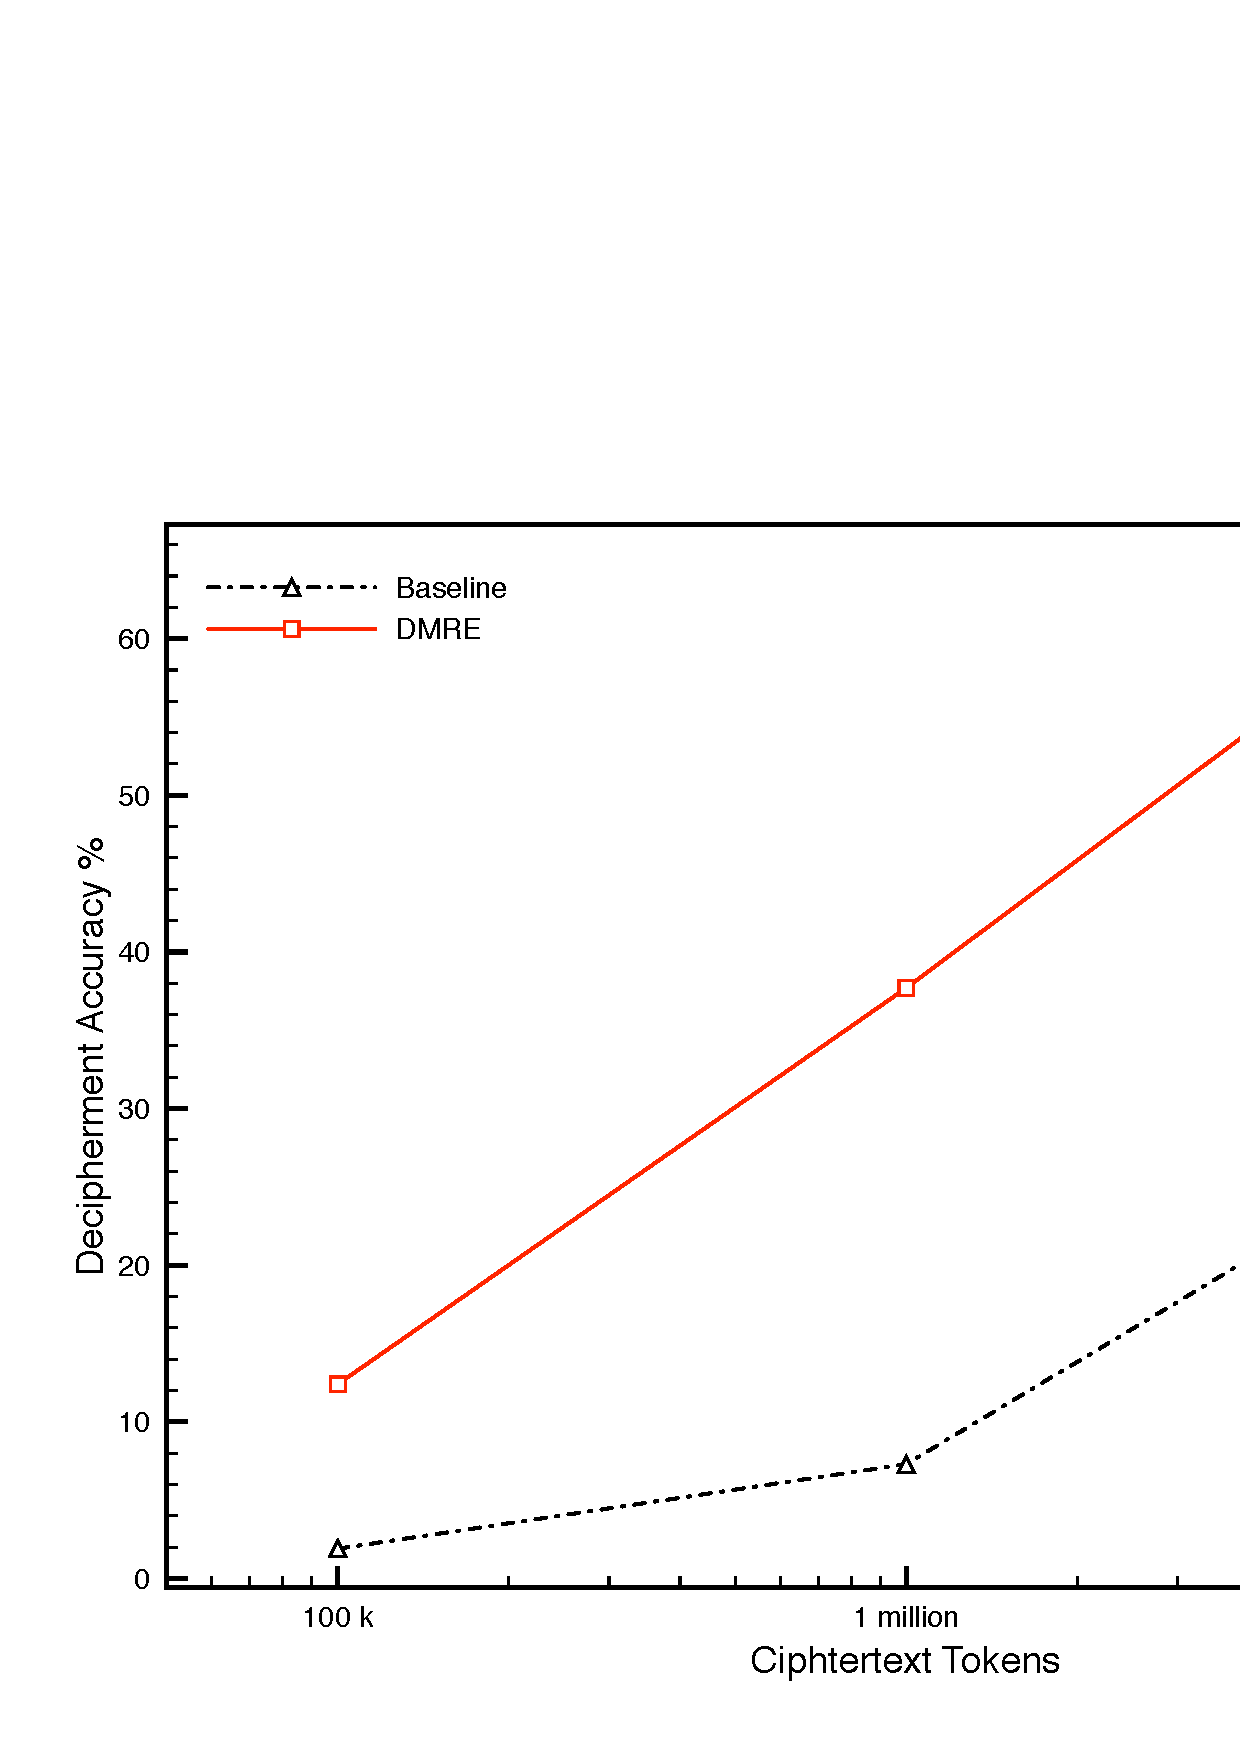
\includegraphics[width=3.1in,height=2.4in]{es_en_curve}
  \caption{Learning curves of top-5 accuracy evaluated on 5k most frequent word types for Spanish/English decipherment.}
\label{es-en-curve}
\end{figure}

We also present the learning curves of decipherment accuracy for the 5k most frequent word types. Figure~\ref{es-en-curve} compares the baseline with \textbf{DMRE} in deciphering Spanish into English. Performance of the baseline is in line with previous work \cite{dou-knight:2013:EMNLP}. (The accuracy reported here is higher as we evaluate top-5 accuracy for each word type.) With 100k tokens of Spanish text, the baseline achieves 1.9\% accuracy, while \textbf{DMRE} reaches 12.4\% accuracy, improving the baseline by over 6 times. The improvement holds consistently throughout the experiment. In the end, the baseline achieves 29.0\% accuracy, while \textbf{DMRE} reaches 64.7\% accuracy, over 2 times higher. 

 \begin{figure}[!ht]
  \centering
  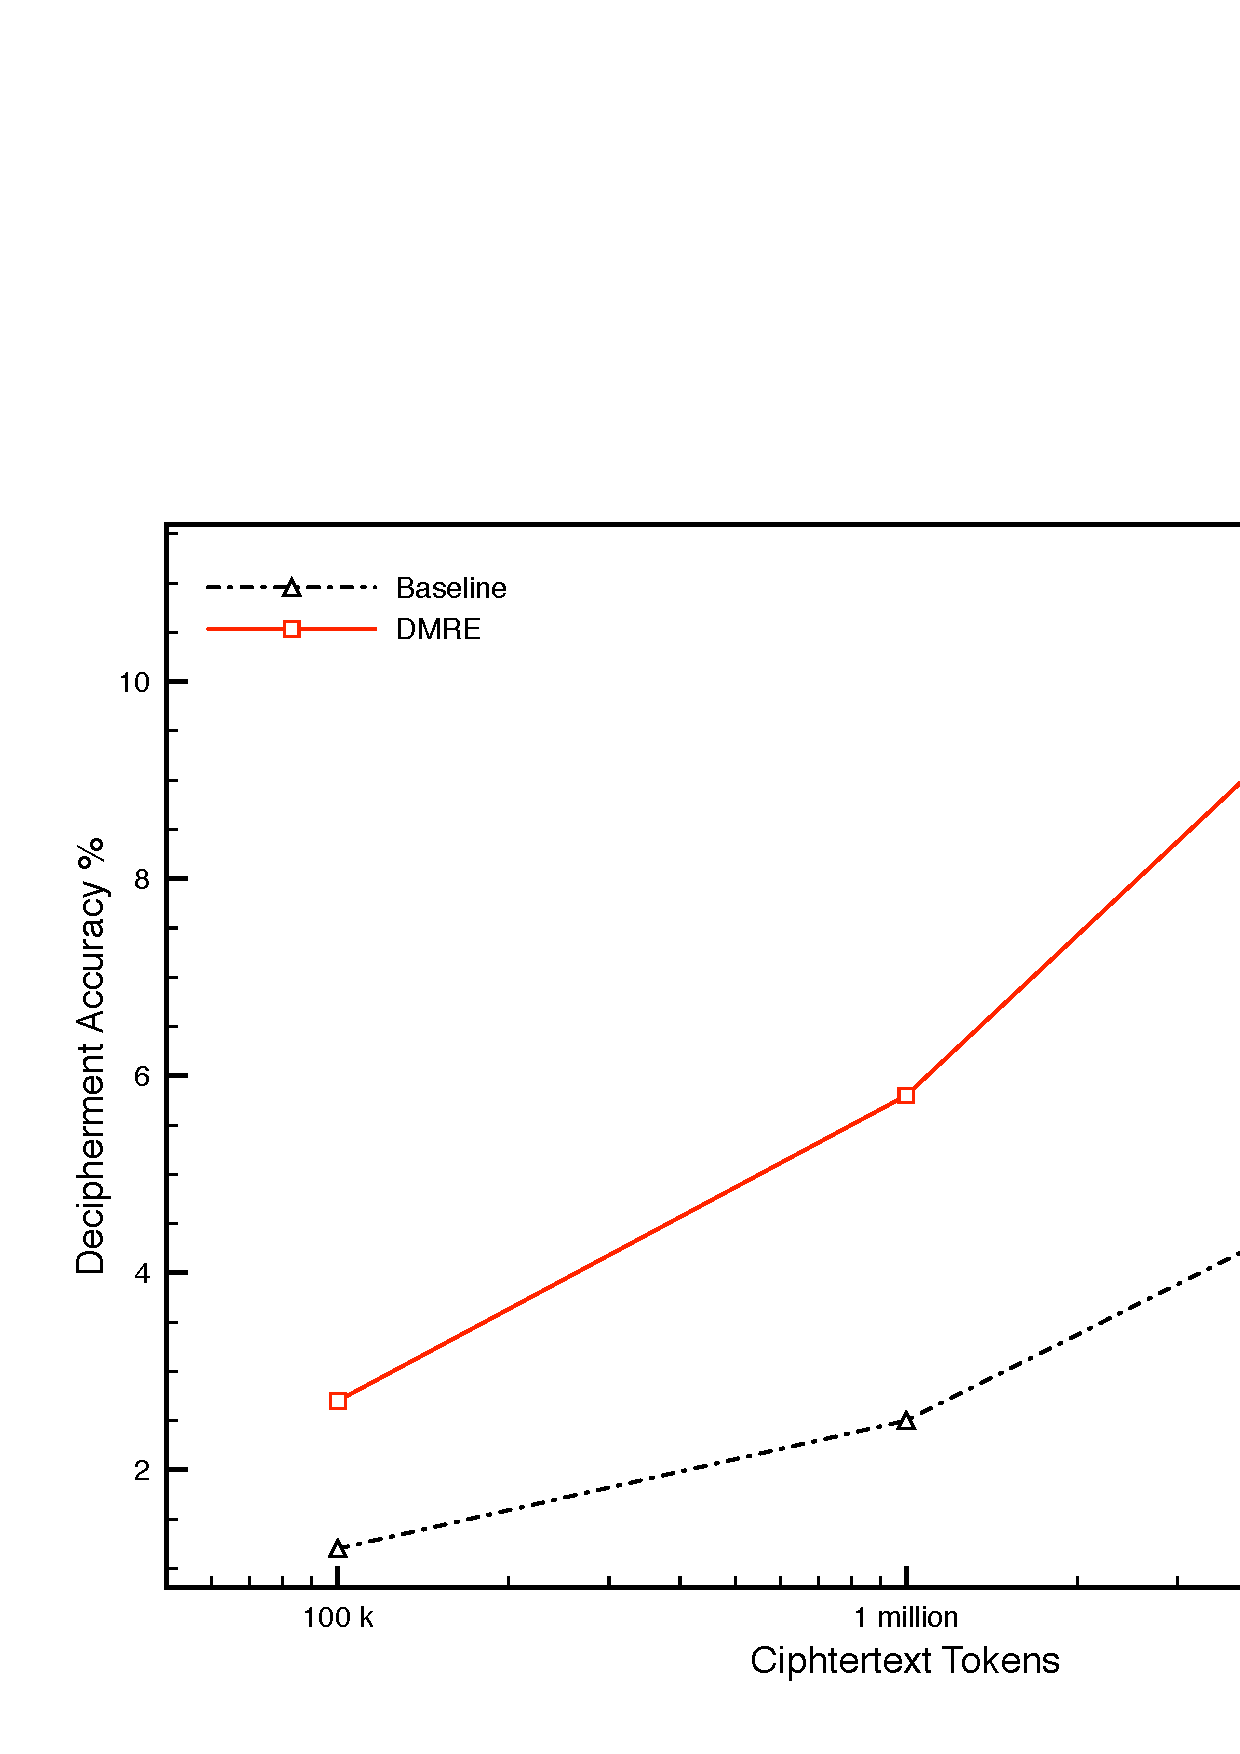
\includegraphics[width=3.1in,height=2.4in]{mlg_en_curve}
  \caption{Learning curves of top-5 accuracy evaluated on 5k most frequent word types for Malagasy/English decipherment.}
\label{mlg-en-curve}
\end{figure}

Figure \ref{mlg-en-curve} compares the baseline with our new approach in deciphering Malagasy into English. With 100k tokens of data, the baseline achieves 1.2\% accuracy, and \textbf{DMRE} improves it to 2.4\%.  We observe consistent improvement throughout the experiment. In the end, the baseline accuracy obtains 5.8\% accuracy, and \textbf{DMRE} improves it to 11.2\%.

Overall, we achieve large consistent gains across both language pairs. We hypothesize the gain comes from a better base distribution that considers larger context information. This helps prevent the language model driving deicpherment to a wrong direction. 

%We evaluate the base distribution with the same translation table we use for evaluation decipherment accuracy. For each cipher word type $f$, if any of its translation $e$ with score $P(e|f) \geq 0.1$ appears in the top 500 candidates proposed by the base distribution, we view that the base distribution proposes a correct translation for $f$. We evaluate base distribution learned during Spanish-English decipherment. The total number of evaluable word types is 7469. With 100k cipher tokens, 5416 are correct, with 10m cipher tokens, 6123 are correct.
Since our learned transformation matrix $M$ significantly improves decipherment accuracy, it's likely that it is \emph{translation preserving}, that is, plaintext words are transformed from their native vector space to points in the ciphertext such that translations are close to each other. To visualize this effect, we take the $5k$ most frequent plaintext words and transform them into new embeddings in the ciphertext embedding space $v_{\plain'} = v_{\plain}^T M$, where $M$ is learned from 10 million Spanish bigram data. We then project the $5k$ most frequent ciphertext words and the projected plaintext words from the joint embedding space into a $2-$dimensional space using t-sne~\cite{van2008visualizing}. 

In Figure~\ref{fig:overlap}, we see an instance of a recurring phenomenon, where translation pairs are very close and sometimes even overlap each other, for example (judge, jueces), (secret, secretos). The word ``magistrado'' does not appear in our evaluation set. However, it is placed close to its possible translations. Thus, our approach is capable of learning word translations that cannot be discovered from limited parallel data. 

We often also see \emph{translation clusters}, where translations of groups of words are close to each other. For example, in Figure~\ref{fig:trans-cluster}, we can see that time expressions in Spanish are quite close to their translations in English. Although better quality translation visualizations~\cite{mikolov2013exploiting} have been presented in previous work, they exploit large amounts of parallel data to learn the mapping between source and target words, while our transformation is learned on \emph{non-parallel} data. 

% A common approach to evaluate mappings between different word-vector spaces is to inspect the joint embedding of words in To show that the base distribution we learned is sensible , we visualize it in Figure \ref{viz_countries} and Figure \ref{viz_close}. To generate the visualizations, we first project English embeddings vectors into Spanish embeddings space using the similarity matrix $M$. Then, we put the word vectors together and project all of them from 50 dimension down to 2 dimension. Two words are close if their embeddings vectors are similar. Ideally, we hope words that are translations are also close to each other.

 \begin{figure}[!ht]
  \centering
  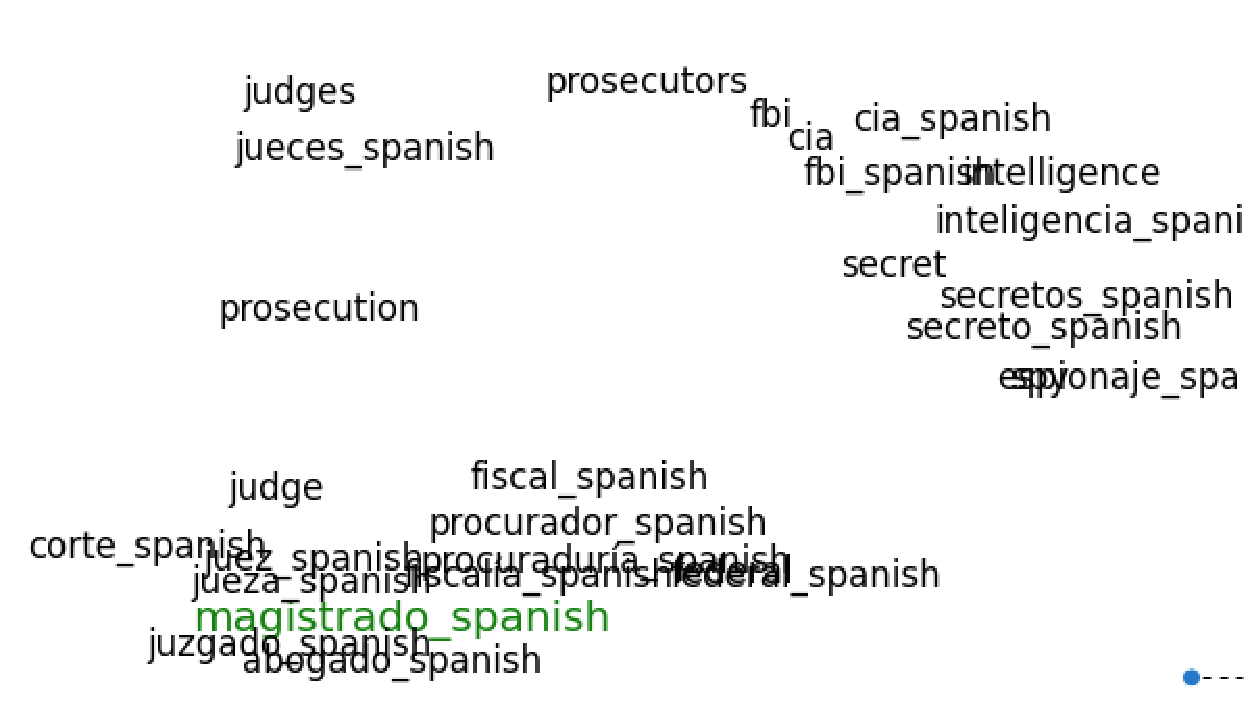
\includegraphics[width=3.0in,height=2.0in]{magistrado}
  \caption{Translation pairs are often close and sometimes overlap each other. Words in spanish have been appended with \_spanish}
\label{fig:overlap}
\end{figure}


 \begin{figure}[!ht]
  \centering
  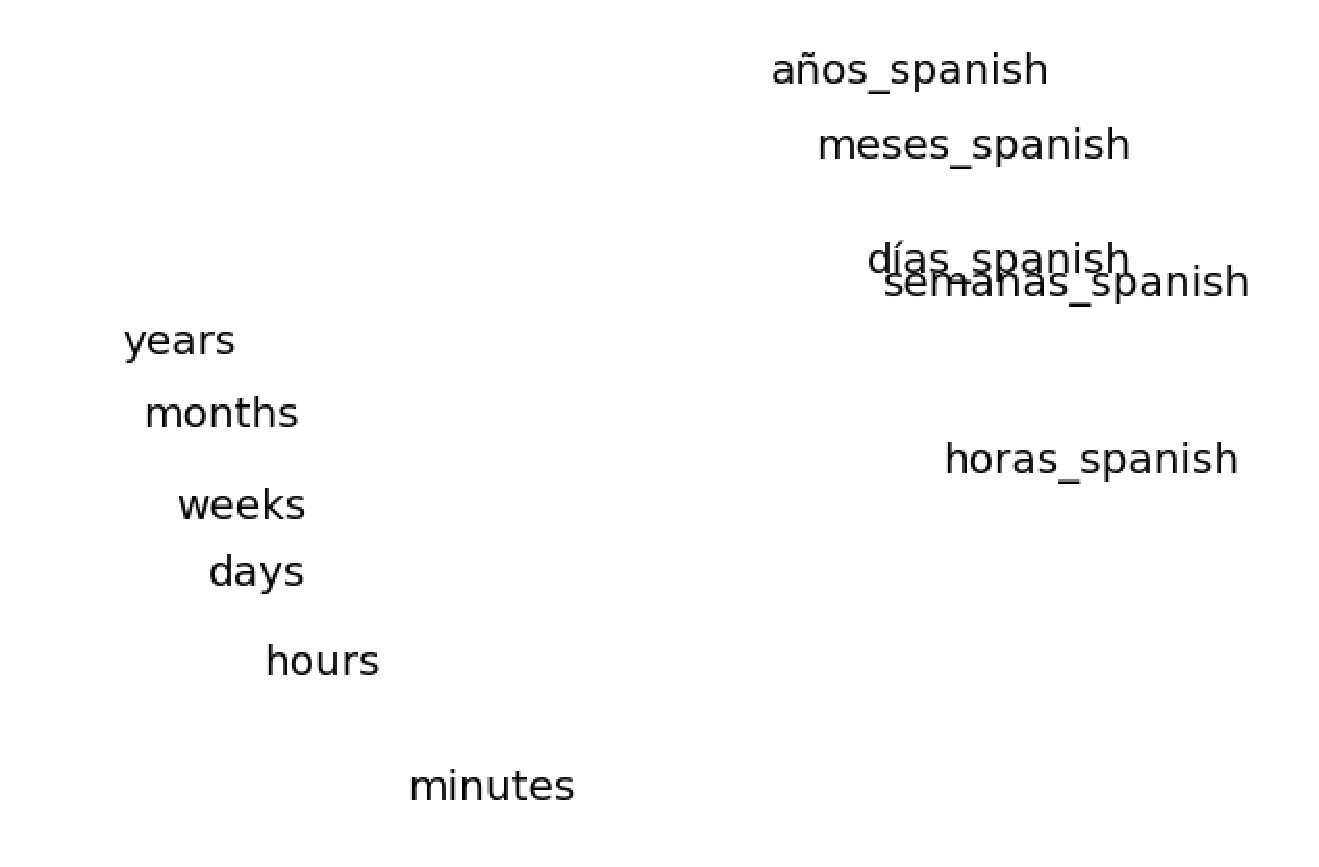
\includegraphics[width=3.0in,height=2.0in]{time}
  \caption{Semantic groups of word-translations appear close to each other.}
\label{fig:trans-cluster}
\end{figure}

%The first thing we observe is that translations appear close as groups. As shown in 
%Fiture \ref{viz_countries}, the group of country names in Spanish and their English translations are near to each other.

These results show that our approach can achieve high translation accuracy and discover novel word translations from non-parallel data. 

%As shown in Figure \ref{viz_close} When we look deeper, we also find many pairs of translations that are right next to each other. Previous work has also produced similar visualization with help of parallel data. However, we learn the mapping using only monolingual data.
